\subsection{Numerical Investigation of Propagating Modes in TEM Cells}
\subsubsection{Theoreticals}
% Goal is to describe the modes in a TEM cell, including their cut-off frequencies. \cite{Kreindl_Bauernfeind_Weiss_Stockreitner_Kaltenbacher_2024} shows that these investigations are important. There are also modes propagating perpendicular to the intended propagation direction. Why are no waveguides used? Explain.

% In this paper, a VCSEL with a decoupling capacitor are modeled. It is visible, that the electric coupling dominates at an orientation of 90°. A local minimum is then visible. At 400\,MHz and upwards, inductive coupling becomes dominant, but only at 0° where it couples with the septum. It is possible, that a certain mode can propagate at a certain frequency, which influenced the result in this paper. 


Any electromagnetic field distribution in a waveguide can be represented by an infinite series of normal modes. \autoref{eqn:norm_power} shows that each mode is orthogonal to each other, with $\mathbf{e_n}^\pm$ and $\mathbf{h_n^\pm}$ being the function vectors of the electric and magnetic field in transverse direction \cite{Collin_2015}. Additionally, each mode carries unit power, shown by \autoref{eqn:unit_power}. Only the transverse fields are investigated in these Equations, because they carry power along the waveguide, opposed to the fields in the propagation direction.

\begin{equation}
    \iint \mathbf{e_n^\pm}\times \mathbf{h_m^\pm}\mathrm{d}S\mathbf{n}=0
    \label{eqn:norm_power}
\end{equation}

\begin{equation}
    \iint \mathbf{e_n^\pm}\times \mathbf{h_n^\pm}\mathrm{d}S\mathbf{n}=1\,\mathrm{W}
    \label{eqn:unit_power}
\end{equation}

Therefore, the radiated fields can be described by superposition of normals modes, as in \autoref{eqn:modal_superposition1} and \autoref{eqn:modal_superposition2}. These modes already consider the boundary conditions of the waveguide, therefore simplifying the calculations. The coefficients of these modes are straightforward to calculate, due to Lorentz Reciprocity Theorem, if the waveguide's walls are perfectly conducting. Also, if the dimensions of the waveguide is small enough, any higher order mode than the first TEM mode will be suppressed. 

\begin{align}
    \mathbf{E^\pm}&=\sum_na_n\mathbf{E_n^\pm}    \label{eqn:modal_superposition1}\\
    \mathbf{H^\pm}&=\sum_na_n\mathbf{H_n^\pm}    \label{eqn:modal_superposition2}
\end{align}

Suppose a current source $\mathbf{J_1}$ excites a waveguide (as is the case with the dipoles in the TEM cell). Normally, such a current source would be driven with external fields, but for the sake of the argument, they are ignored. Only $\mathbf{E}$ and $\mathbf{H}$ are considered, which are the fields radiated by $\mathbf{J_1}$. Additionally, $\mathbf{E_n^\pm}$ and $\mathbf{H_n^\pm}$ are the resulting transverse waveguide fields, with the signs indicating the direction of propagation. Take \autoref{eqn:lorentz_rec_theorem_int} and set $\mathbf{J_2}=\mathbf{M_1}=\mathbf{M_2}=0$. Now, only the current source $\mathbf{J_1}$ remains, and the \autoref{eqn:J1_propagating_waves} emerges. % Explain how certain surfaces do not to have be integrated, therefore rendering this equation very useful. Also, the expansion coefficients can be determined. Maybe do this calculation with a rectangular waveguide.

\begin{equation}
    \oiint _S (\mathbf{E_n^\pm}\times \mathbf{H}-\mathbf{E}\times \mathbf{H}_n^\pm)\cdot\mathrm{d}\mathbf{S}=\iiint \mathbf{J_1}\cdot\mathbf{E_n^\pm}\mathrm{d}V
    \label{eqn:J1_propagating_waves}
\end{equation}

\subsubsection{Modes in TEM cell}

A TEM cell is often used for EMC test specifications, as it enables the propagation of TEM waves, which resemble planar free-space waves. A simple rectangular waveguide cannot be used for this application, as shall be shown here. % Continue with some calculations, showing that TEM wave propagation is not possible?

The TEM cell does not only support TEM modes, above their cut-off frequency TE and TM modes begin to propagate. Because the TEM cell is a high-Q cavity, those cut-off frequencies are sharply defined frequencies. A paper by Wilson and Ma present analytical approximations to determine these frequencies \cite{Wilson_Ma_1986}.  There is a long list for the several first few corner frequencies of the first modes.

\begin{figure}[h]
    \centering
    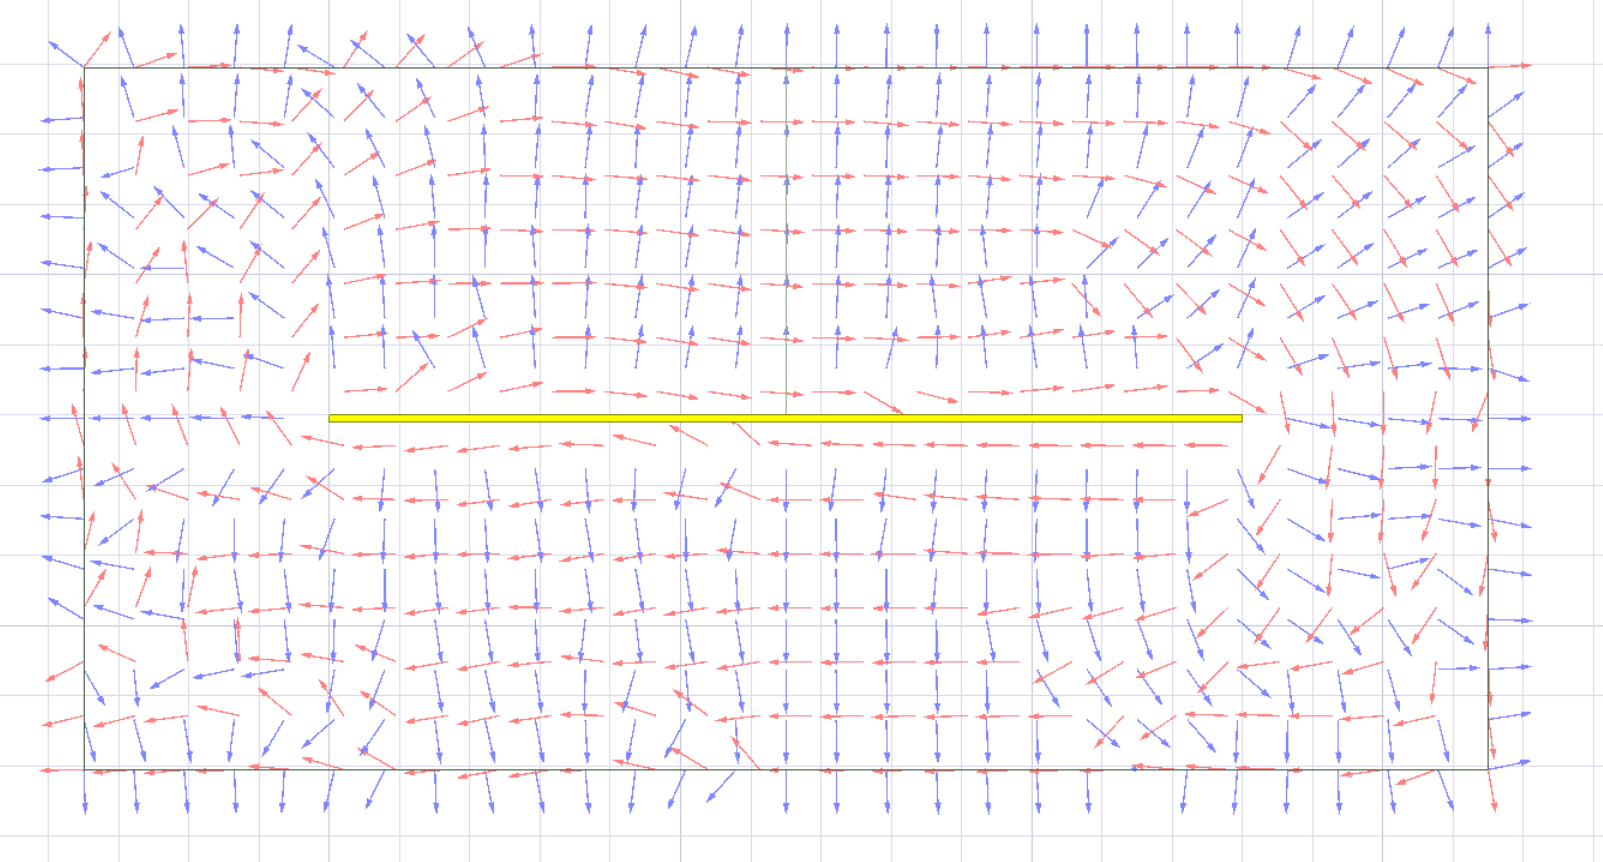
\includegraphics[width=0.5\linewidth]{images/tem_mode.png}
    \caption{TEM Mode}
    \label{fig:tem_mode}
\end{figure}
%(My TEM cell is too short to have more modes than this) Investigation of more modes would be interesting

The first mode after the TEM mode is the TE\textsubscript{01}

